\section{Rauschen}
\vspace{-3mm}
\begin{longtable}{|p{3.5cm}|p{6cm}|p{8cm}|}
	\hline
    \multicolumn{3}{|l|}{\bf Typen von Rauschen}
    \\ \hline
	Shot / Schottky / quantum noise
	& \vspace{-1.5\topsep}
      \begin{itemize}[leftmargin=*]
  		\item Verursacht durch zufällige Fluktuationen der Bewegung von Ladungsträgern, die Potentialbarrieren überwinden müssen
  		\item Charakteristik
  		\begin{itemize}
    		\item geknüpft an Stromfluss
    		\item Unabhängig von Temperatur
    		\item Spektral "`flach"'
    	\end{itemize}
	  \end{itemize}
	& {
		$E_{sh}=kT\sqrt{\frac{2B}{qI_{dc}}}$\newline
		$E_{sh}= 0.4\mu V @ 1mA,1MHz$\newline
        
		k: Bolzmannkonstante ($1.38 \cdot 10^{-23}$Joule/$^\circ$K)\newline
		q: Elektronenladung ($1.6 \cdot 10^{-19}$Coulomb)\newline
		T: Temperatur in $^\circ$K\newline
		$I_{dc}$: Durchschnittlicher DC Strom in A\newline
		B: Bandbreite in Hz
      }
	\\ \hdashline
	Thermisches Rauschen
	& Konstant für alle Frequenzen
	&
	\\ \hdashline
	Flicker Noise, 1/f noise, rosa Rauschen
	& \vspace{-1.5\topsep}
      \begin{itemize}[leftmargin=*]
	  	\item nicht gleichverteilt über die Frequenz, seine
  	  	\item Rauschleistung nimmt umgekehrt proportional zur Frequenz ab.
  	  \end{itemize}
  	& {\begin{gather*}
		E_{n}=K_{v}\sqrt{\ln{\frac{f_{max}}{f_{min}}}}\\
		I_{n}=K_{i}\sqrt{\ln{\frac{f_{max}}{f_{min}}}}
  	  \end{gather*}}\\
	\hline    
\end{longtable}
% ----------------------------------------------------------------------------------------------------
\vspace{-2.5\topsep}
\begin{longtable}{|p{4.27cm}p{4.27cm}|p{4.27cm}p{4.27cm}|}
    \hline
    \multicolumn{4}{|l|}{\bf Rausch-Farben}
    \\ \hline
    \textbf{Color} & \textbf{Frequency Spectrum} & \textbf{Color} & \textbf{Frequency Spectrum}
    \\ \hline
    Purple         & $\mathrm{f^2}$              & Blue           & f\\
    White          & 1                           & Pink           & $\mathrm{\frac{1}{f}}$\\
    Red/Brown      & $\mathrm{\frac{1}{f^2}}$    &                & \\
    \hline
\end{longtable}
% ----------------------------------------------------------------------------------------------------
\vspace{-2.5\topsep}
\renewcommand{\arraystretch}{1.8}
\begin{longtable}{|p{5cm}|p{12.9cm}|}
    \hline
    \multicolumn{2}{|l|}{\bf Leistung des Rauschens}
    \\ \hline
    Mittelwert	
    & $\overline{\nu_{n}}(t)\leq \nu_{n}(t)\geq \frac{1}{T}\int_{T}\nu_{n}(t)dt=0$ 
    \\ \hline
    Varianz (Leistung)
    & $\overline{\nu_{n}}(t)^2=\frac{1}{T}\int_{T}\nu^2_{n}(t)dt\neq0$
    \\ \hline
    Effektivwert
    & $\nu_{n,rms}=\sqrt{\overline{\nu_{n}(t)^2}}$
    \\ \hline
    \multicolumn{2}{|l|}{\parbox{17.9cm}{\vspace{2mm}
        Rechnen mit Rauschen: \textcolor{red}{Signale und Rauschen addieren sich nicht gleich}:
        \begin{itemize}
            \item deterministische Signale: Amplituden addieren sich
            \item statistisch unabhängige Rauschquellen: Rauschleistung addiert sich
        \end{itemize}\vspace{2mm}}}
    \\ \hline
\end{longtable}
% ----------------------------------------------------------------------------------------------------
\vspace{-2.5\topsep}
\begin{longtable}[t]{|p{4cm}|p{6.5cm}|p{7cm}|}
    \hline
    \multicolumn{3}{|l|}{\bf Rauschen von Widerständen}
    \\ \hline
    \multicolumn{3}{|l|}{\textit{Strom- und Spannungsrauschen}}
    \\ \hdashline
    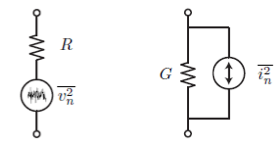
\includegraphics[width=4cm, valign=t]{pictures/widerstandrauschen.png}
    & {	\vspace{-1.8\topsep}
        \begin{align*}
            S_{noise}(R) &=4kTR\\
            E_{noise}(R) &=\sqrt{4kTR}\\
            \overline{\nu^2_{n}} &=4kTRB = \int 4kTR \; df\\
            \overline{i^2_{n}} &=4kTGB = \int 4kTG \; df\\
            \nu_{rms} &= \sqrt{\overline{\nu^2_{n}}} = \sqrt{4kTRB}
        \end{align*}
      }
    & {B: Bandbreite\newline
       T:  Temperatur in Kelvin(293K)\newline
       k:  $1.38 \cdot 10^{-23}JK^{-1}$\newline
       $S_{noise}(R)$:  Spektrale Dichte (Leistung)\newline
       $E_{noise}(R)$: Rauschspannungsdichte\newline
       $\nu_{RMS}$:  Rauschspannung
      }
    \\ \hline
% ----------------------------------------------------------------------------------------------------   
    \multicolumn{3}{|l|}{\textit{Widerstände in Serie}}
    \\ \hdashline
    \begin{circuitikz}[european, scale=2]
	\draw (0,0) to [R=$R1$, *-] (1,0) to [R=$R2$, -*] (2,0);
\end{circuitikz}
    & {	\vspace{-1.6\topsep}
        \begin{align*}
            \overline{\nu^2_{n}}&=4kT(R1+R2)B=\overline{\nu^2_{n1}}+\overline{\nu^2_{n2}}\\
            \overline{i^2_{n}}&=4kT(G1+G2)B=\overline{i^2_{n1}}+\overline{i^2_{n2}}
        \end{align*}
    }
    & {\textcolor{red}{\bf Nicht die Rausch-Spannungen, sondern die Rausch-Leistungen müssen addiert werden!}
    }
    \\ \hline
\end{longtable}
% ----------------------------------------------------------------------------------------------------  
\begin{longtable}[t]{|p{4cm}|p{5.2cm}|p{7cm}|}    
    \hline 
    \multicolumn{3}{|l|}{\textit{Spannungsteiler}}
    \\ \hdashline
    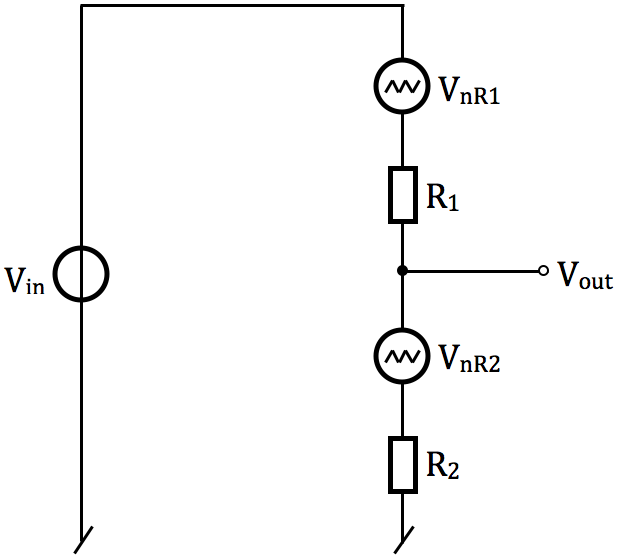
\includegraphics[width=4cm, valign=t]{pictures/RauschenSpannungsteiler.png}
    & {\begin{align*}
            \intertext{Superposition der einzelnen Spannungsquellen}
            V_{out}(V_{in}) &= V_{in} \cdot \frac{R_2}{R_1 + R_2}\\
            V_{out}(V_{nR1}) &= V_{nR1} \cdot \frac{R_2}{R_1 + R_2}\\
            V_{out}(V_{nR2}) &= V_{nR2} \cdot \frac{R_1}{R_1 + R_2}
        \end{align*}
      }
    & {\begin{align*}
            \intertext{\textcolor{red}{Nicht Rauschspannungen, sondern Leistungen addieren}}
            V_{n_{out}}^2 &= \left[ S_{R_1}\left( \frac{R_2}{R_1 + R_2}\right) ^2 + S_{R_2}\left( \frac{R_1}{R_1 + R_2}\right) ^2\right] B \\
            &= 4kT\left( R_1 \frac{R_2^2}{(R_1+R_2)^2} + R_2 \frac{R_1^2}{(R_1+R_2)^2}\right) B\\
            V_{n_{out}} &= \sqrt{\mathrel{\mathop{V_{nR1}^2}\limits_{\substack{\uparrow\\\hbox to 0pt{\hss{\textcolor{red}{\tiny $4kT R_1 B$}}\hss}}}} \left( \frac{R_2}{R_1+R_2}\right) ^2 + \mathrel{\mathop{V_{nR2}^2}\limits_{\substack{\uparrow\\\hbox to 0pt{\hss{\textcolor{red}{\tiny $4kT R_2 B$}}\hss}}}} \left( \frac{R_1}{R_1+R_2}\right) ^2}
        \end{align*}
      }
    \\ \hdashline
    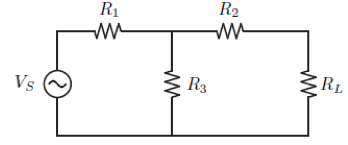
\includegraphics[width=4cm, valign=t]{pictures/seriewiderstand1.png}\newline
    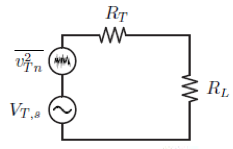
\includegraphics[width=4cm]{pictures/seriewiderstand2.png}
    & {Quellenumwandlung machen und dann Rauschen über Ersatzwiderstand ($R_T$) bestimmen.\newline
       \begin{align*}
           V_{T,s}&=V_{s}\frac{R_{3}}{R_{1}+R_{3}}\\
           \overline{\nu^2_{Tn}}&=4kTR_{T}B\\
           &=4kT(R_{2}+R_{1}\parallel R_{3})B
       \end{align*}
      }
    & {
      }
    \\ \hline
% ----------------------------------------------------------------------------------------------------       
    \multicolumn{3}{|l|}{\textit{Rauschen von RC-Netzwerken}}
    \\ \hdashline
    \begin{center} \begin{circuitikz}[european]
	\ctikzset{bipoles/length=1cm}
	\draw (0,0) node[ocirc] {} 
		to[short] ++(1,0) node[circ] {}
		to[short] ++(1.3,0)
		to[C=C] ++(0,-1.5)
		to[short] ++(-1.3,0) node[circ] {}
		to[short] ++(-1,0) node[ocirc] {};
	\draw (1,0) to[R=G] (1,-1.5);
	\draw[->] (-0.2,-1.9) node[below] {$\underline{Z}$} -- ++(0,1.2) -- ++(0.4,0);
\end{circuitikz} \end{center}
    & { \vspace{-1.5\topsep}
        \begin{align*}
            Z &=\frac{1}{Y}=\frac{1}{G+j\omega C}=\frac{G-j\omega C}{G^2+\omega^2C^2}\\
            \overline{\nu^2_{n}} &=\frac{4kT}{2\pi}\int^{\infty}_{0}\frac{G}{G^2+\omega^2C^2}d\omega=\frac{kT}{C}\\
            \overline{\nu_{n}} &=\sqrt{\frac{kT}{C}}
        \end{align*}
      }
    & {\vspace{-1.5\topsep}
        \begin{itemize}[leftmargin=*]
            \item Kapazitäten (und Induktivitäten) rauschen nicht!
            \item Kapazitäten (und Induktivitäten) ändern die Bandbreite des Systems, d.h. beeinflussen dadurch die Rauschspannung
            \item Der Widerstand trägt nicht direkt zur Rauschspannung bei, er limitiert die Bandbreite
            \newline
        \end{itemize}
      }
    \\ \hline
\end{longtable}
% ----------------------------------------------------------------------------------------------------    
\vspace{-2.5\topsep}
\begin{longtable}[t]{|p{4cm}|p{5.5cm}|p{7.8cm}|}
    \hline  
    \multicolumn{3}{|l|}{\bf Berechnung der Rausch-Spannung}
    \\ \hdashline
    Die Rausch-Spannung ist das Integral der Rauschspannungsdichte über den ganzen Frequenzbereich
    & {\vspace{-1.5\topsep}
       \begin{align*}
            \intertext{für weisses Rauschen}
            \overline{e^2} &= \int_{f_L}^{f_H} C \, df = \underbrace{C}_{4kT\cdot R} (f_H-f_L) \\
            \intertext{für 1/f-Rauschen}
            \overline{e^2} &= \int_{f_L}^{f_H} \frac{K^2}{f} \, df = K^2 \ln\frac{f_H}{f_L}
       \end{align*}
      }
    & {C: Rauschleistungsdichte pro Hertz (konstant)\newline
       \newline\newline\newline
       K: Bauteil-Konstante (in Volt)
      }
    \\ \hline
\end{longtable}
\newpage
% ----------------------------------------------------------------------------------------------------    
\vspace{-2.5\topsep}
\begin{longtable}[t]{|p{4cm}|p{8cm}|p{5.3cm}|}
    \hline  
    \multicolumn{3}{|l|}{\bf Berechnung der Rausch-Bandbreite (am Beispiel von Tiefpass 1. Ordnung)}
    \\ \hdashline
    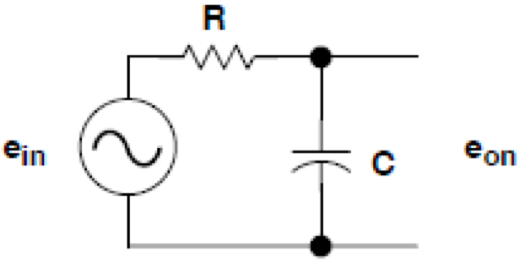
\includegraphics[width=4cm, valign=t]{pictures/RauschenTiefpass.png}
    & {\vspace{-1.5\topsep}
        \begin{align*}
            e_{on} &= \sqrt{\int_{0}^{\infty} \left| A_{n(f)}\right| ^2 e_{in}^2 \, df}\\
            A_{n(f)} &= \frac{1}{1+ j2\pi fRC} \Rightarrow \left| A_{n(f)}\right| ^2 = \frac{1}{1+(2\pi fRC)^2}\\
            e_{on} &= e_{in} \sqrt{\int_{0}^{\infty} \frac{1}{(2\pi fRC)^2}df} = e_{in} \sqrt{\underbrace{\frac{1}{2\pi RC}\frac{\pi}{2}}_{\textcolor{red}{ENB}}}
        \end{align*}
        \begin{tabbing}
            {\bf Filter-Ordnung}\qquad \= {\bf ENB}\\
            1 \> $1.57 \cdot f_c$\\
            2 \> $1.11 \cdot f_c$\\
            3 \> $1.05 \cdot f_c$\\
            4 \> $1.025 \cdot f_c$
        \end{tabbing}
      }
    & {$\mathrm{\bf e_{on}}$: Rauschspannung am Ausgang der Schaltung\newline\newline
       $\mathrm{\bf e_{in}}$: Rauschspannung am Eingang der Schaltung\newline\newline
       {\bf \textcolor{red}{ENB}}: Effective Noise Bandwidth\newline
       Es wird nicht die 3dB-Bandbreite, sondern das gesamte integrierte Rauschen berechnet
      }
    \\ \hline
\end{longtable}
% ----------------------------------------------------------------------------------------------------    
\vspace{-2.5\topsep}
\begin{longtable}[t]{|p{4cm}|p{13.7cm}|}
    \hline  
    \multicolumn{2}{|l|}{\bf Rauschen in Opamps}
    \\ \hdashline
    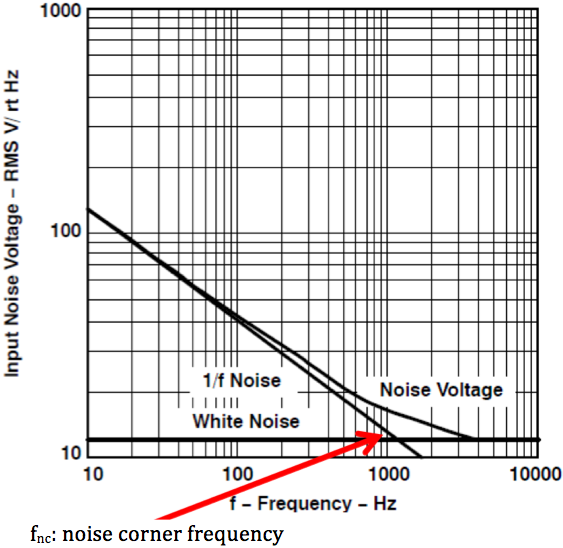
\includegraphics[width=4cm, valign=t]{pictures/NoiseCornerFreq.png}\newline\newline
    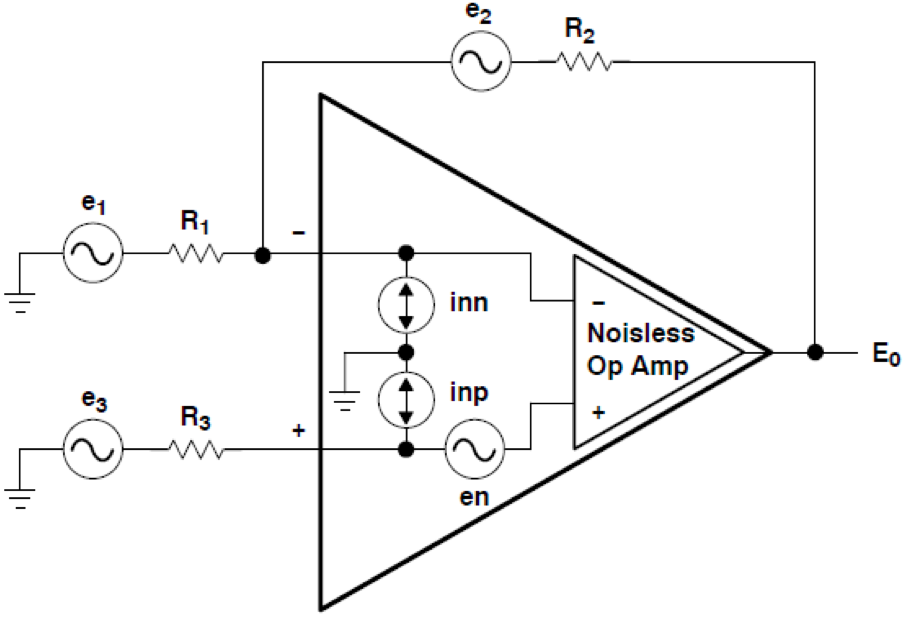
\includegraphics[width=4cm]{pictures/oampnoise.png}
    & {Bei $\mathrm{f_{nc}}$ kreuzt das 1/f-Rauschen mit dem weissen Rauschen\newline
       Gesamtrauschen: $\overline{E^2} = C\left( f_{nc} \ln \frac{f_H}{f_L} + f_H - f_L\right) $\newline
       \begin{align*}
           E_{Trms}=&\sqrt{\int 4kTR_2\left( \frac{R_1+R_2}{R_1}\right) + 4kTR_3\left( \frac{R_1 + R_2}{R_1}\right) ^2 + ((i_{nn})R_2)^2 + \dots}\\
           &\overline{\dots \left( (i_{np})R_3\left( \frac{R_1+R_2}{R_1}\right) \right) ^2 + \left( e_n\left( \frac{R_1+R_2}{R_1}\right) \right) ^2 df}
       \end{align*}
       \newline
       \textbf{Vereinfacht für CMOS-Opamps:} \newline
       \vspace{-1.5\topsep}
       \begin{itemize}[leftmargin=*]
           \item $R_3=0$
           \item Gain A = $\frac{R1+R2}{R1}$
           \item $e_w$: Noise/$\sqrt{Hz}$ (aus Datenblatt)
           \item $f_{nc}$: noise corner frequency (aus Datenblatt)
           \item \textcolor{red}{ENB}: Effective Noise Bandwidth
           \newline
        \end{itemize}
       $E_{Trms}=\sqrt{\textcolor{red}{ENB} \cdot 4kTR_2 A+e_w^2 A^2\cdot (f_{nc}\cdot \ln{\frac{f_{H}}{f_{L}}}+\textcolor{red}{ENB})}$\newline
       Ist die Bandbreite $>>f_{enc}$ ( mind. 10x grösser) kann 1/f-Noise vernachlässigt werden\newline
       \vspace{-1.5\topsep}
       \begin{itemize}[leftmargin=*]
           \item Gain $A=\frac{R1+R2}{R1}$
           \item $e_w$: Noise/$\sqrt{Hz}$ (aus Datenblatt)
           \item \textcolor{red}{ENB}: Effective Noise Bandwidth ($1.51 \cdot \frac{GBW}{A}$)
           \newline
        \end{itemize}
        $V_{noise}=\sqrt{4kT \cdot R_{2} \cdot A \cdot \textcolor{red}{ENB}+e_{w}^2 \cdot A^2 \cdot \textcolor{red}{ENB}}$
    }
    \\ \hline
\end{longtable}
